\chapter{Validating structural predictions of conjugated macromolecules in Espaloma-enabled reproducible workflows}
The following chapter contains yet to be published work written by me with the guidance of Dr. Eric Jankowski. The following work has been submitted to the International Journal of Molecular Sciences and is expected to be published in Januaray 2025.
\label{chap:EspVal}

\section{Abstract}
We incorporate \texttt{Espaloma} forcefield parameterization into  \texttt{MoSDeF} tools for performing molecular dynamics simulations of organic molecules with \texttt{HOOMD-Blue}. 
We compare equilibrium morphologies predicted for perylene and poly-3-hexylthiophene (P3HT) with the \espff~forcefield in the present work against prior work using the \texttt{OPLS-UA} forcefield. 
We find that after resolving chemical ambiguities in molecular topologies, \espff~is similar to \texttt{GAFF}.
We observe clustering/melting phase behavior to be similar between \espff~and \oplsff, but that the base energy unit of \oplsff~better connects to experimentally-measured transition temperatures.
Short-range ordering measured by radial distribution functions is essentially identical between the two forcefields, and long-range ordering measured by grazing incidence x-ray scattering is qualitatively similar, with \espff~matching experiments better than \oplsff.
We conclude that \texttt{Espaloma} offers promise in the automated screening of molecules from more complex chemical spaces.
%%%%%%%%%%%%%%%%%%%%%%%%%%%%%%%%%%%%%%%%%%%%%%%%%%%%%%%%%%%%%%%%
\section{Introduction}
Molecular simulations offer promise for the high-throughput screening of thermodynamically stable structures from families of molecules.
Such screening studies can identify chemistries and conditions where self-assembly of desired structures are optimized, and can provide insight into identifying chemistry-structure-property relationships that are otherwise inaccessible with experimental methods\cite{daglar_opportunities_2020,liu2018molecular,lin2020review,afzal2020high,meier2004combinatorial,quach2022high}.
One challenge of screening studies, particularly of polymers, is that the parameters that define the interactions between and within model molecules may not have been defined for a given ``off-the-shelf'' forcefield\cite{wang_end--end_2022}. 
In molecular mechanics simulations, forcefields define the potential energies and therefore forces of bond, angle, torsion/dihedral, and non-bonded models of interatomic interactions\cite{hopfinger1984molecular,vanommeslaeghe2014molecular}. 
For example, the popular Optimized Potentials for Liquid Simulations (OPLS) forcefield has mainly been built around simulating hydrocarbons and proteins \citep{opls,ghahremanpour_refinement_2022}.
The General Amber forcefield (GAFF) is optimized for small organic molecules\cite{wang2004development}.

An example of missing parameters arises when attempting to simulate the popular organic semiconductor poly(3-hexylthiophene) (P3HT).
When using OPLS, we find the forcefield is missing parameter definitions for hydrogen-carbon-carbon-sulfur (H-C-C-S) dihedrals. 
In such cases, the simulator typically has had two options: (1) they might reuse a similar parameterization from a forcefield based on their chemical intuition, or (2) they can perform quantum chemical calculations to identify new forcefield parameters\cite{hopfinger1984molecular} that best fit the calculated potential energies.
The former option has the downside of missing important physics and giving inaccurate results, while the latter option requires additional software fluency and calculation time\cite{wang_end--end_2022}.
Both options suffer from an additional shortcoming: the forcefields that result are \textit{different} from the forcefields from which they were derived, which complicates data provenance and reproducibility.

Recent efforts towards making simulations more transparent, reproducible, usable, and extensible (TRUE)\cite{thompson2020towards,jankowski2020perspective} have identified programmatic workflows as a best practice.
In the present context, this means that simulation scripts that fully specify forcefields contribute to more reproducible simulations, even if the forcefields are custom derivatives of prior work\cite{Klein_foyer}.
Quantum chemical calculations could therefore be included into the programmatic specification of custom forcefields and in principle be shared as reproducible workflows.

However, re-running quantum chemical calculations itself introduces software dependency issues and extended runtimes that are redundant.
A new tool that ameliorates this problem is \esp, which is an open-source package that uses graph neural networks to perceive chemical environments in a molecular graph and predict molecular mechanics forcefield parameters \citep{wang_end--end_2022}. 
\texttt{Espaloma} was designed for the investigation of biopolymers and has been used to accurately simulate them \citep{shirts2023, takaba_machine-learned_2024}. 
Of central importance to the present work is \esp's promise to programmatically ``fill in'' missing parameters for organic macromolecules and polymers, enabling more TRUE screening studies without extra quantum chemical calculations (Step 3 of \autoref{MD-Diagram}).

Here, we evaluate \esp~for the modeling of highly conjugated macromolecules.  
We generate forcefield parameters using \esp~and compare them to the ``off-the-shelf'' \texttt{OPLS-UA} and \texttt{GAFF} forcefields where possible.
We compare phase diagrams and morphologies from prior work to validate and quantify \esp's predictive capabilities outside its core training set \citep{wang_end--end_2022}. 
A schematic of the MD workflow we implemented in this work is shown in \autoref{MD-Diagram}. 
\begin{figure}
    \centering
    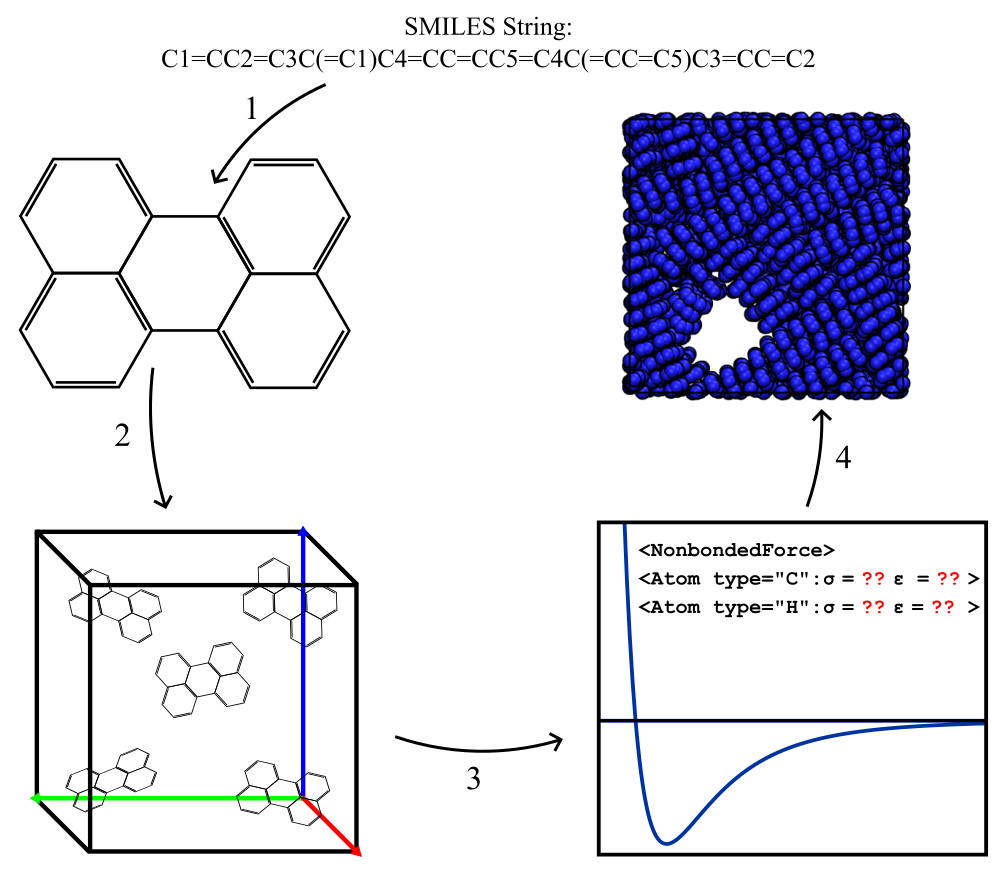
\includegraphics[width=.6\linewidth]{src/figures/FF_figs/MD_process.png}
    \caption{Depictions of our generalized molecular dynamics workflow. Step 1 shows the creation of an \texttt{mBuild Compound} from a SMILES string. In step 2 we create our simulation object using \texttt{flowerMD} and \texttt{PACKMOL}. We employ \esp to parameterize our molecules in step 3 and write the forcefield file. In step 4 we initialize the \texttt{HOOMD-Blue} simulation and predict the morphology of our molecules.}
    \label{MD-Diagram}
\end{figure}


%%%%%%%%%%%%%%%%%%%%%%%%%%%%%%%%%

\section{Model}
We consider united-atom (UA) representations of perylene and P3HT, omitting long-range electrostatics as in prior work\cite{miller_enhanced_2017,miller_optimization_2018}.
Spherical simulation elements are used to represent each ``heavy'' atom and its bonded hydrogens.
Here, the heavy atoms are carbon and sulfur, topologically connected as in \autoref{per_p3ht_fig}.
\begin{figure}[hbt!]
    \centering
    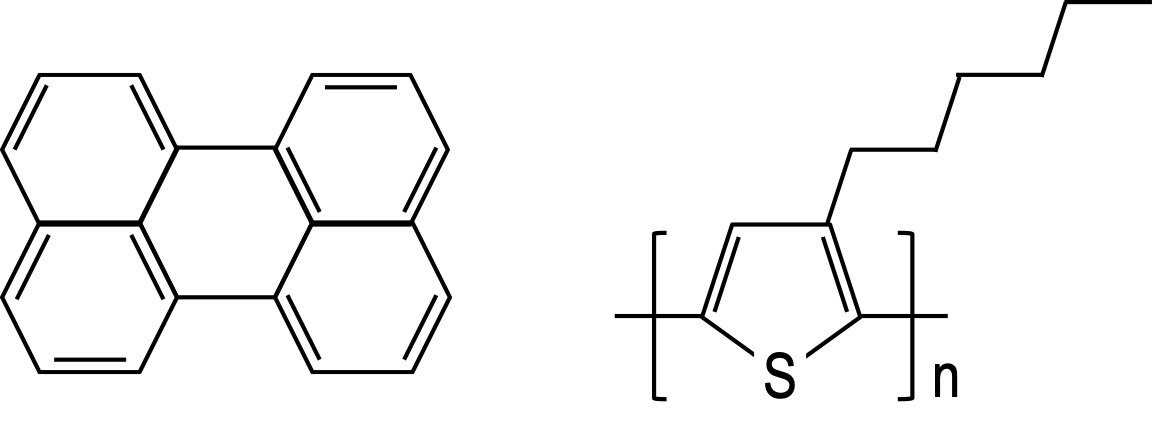
\includegraphics[width=0.6\textwidth]{src/figures/FF_figs/P3HTandPerylene.png} %
    \caption{Diagram of perylene molecule (left) and poly-3-hexylthiophene (P3HT) monomer (right).}
    \label{per_p3ht_fig}
\end{figure}
Chains of $n=15$ repeat units are used to represent P3HT oligomers.
Harmonic potentials are used to model bond-stretching (\autoref{eq:bonds}) and angle bending (\autoref{eq:angles}) between pairs and triplets of bonded atoms. $E_{bonds}$ is the potential energy of a bond, $K_r$ is the bond's harmonic spring constant, $r$ is the internuclear distance, and $r_{eq}$ is the equilibrium internuclear distance. 
\begin{equation}
    E_{bonds} = K_r (r-r_{eq})^2
\label{eq:bonds}
\end{equation}
$E_{angle}$ is the potential energy of a bond angle, $K_{\theta}$ is the harmonic angle constant, $\theta$ is the bond angle, and $\theta_{eq}$ is the equilibrium bond angle. 
\begin{equation}
    E_{angles} = K_{\theta}(\theta-\theta_{eq})^2
\label{eq:angles}
\end{equation}

Cosine series are used to model proper dihedrals (\autoref{eq:dihedrals}) across quadruplets of bonded atoms, where $E_{dihedral}$ is the potential energy of the dihedral, $K_n$ is the force constant of the corresponding particle, $n$, $\phi$ is the dihedral angle, and $\gamma$ is the phase angle. 

\begin{equation}
    E_{dihedral} = \sum_{n=1}^{4}\frac{K_{n}}{2}[1+\cos{(n\phi-\gamma)}]
\label{eq:dihedrals}
\end{equation}

\begin{equation}
    E_{LJ}(r_{i,j}) = 4\epsilon_{i,j} \left[ \left({\frac{\sigma_{i,j}}{r_{i,j}}}\right)^{12} - \left({\frac{\sigma_{i,j}}{r_{i,j}}}\right)^{6} \right] % TODO: This isn't right. Vn aren't defined, nor is gamma, and the LJ potential isn't correct. 
    \label{eq:pairs}
\end{equation}

Simulation elements that are not bonded or separated by more than three bonds within a molecule interact only via the 12-6 Lennard-Jones potential (\autoref{eq:pairs}) \cite{lennard-jones_electronic_1929} truncated at $r_{cut}=2.5\sigma$, where $\sigma$ is the length unit corresponding to the largest simulation element being represented.
Here, this corresponds to sulfur (S) simulation elements for P3HT ($\sigma=3.565$\AA), and carbon (C1) elements for perylene ($\sigma=3.380$\AA).
We apply the Lorentzian combination rule for sigma and a geometric combination rule for epsilon, shown in \autoref{comb_rules}. 
\begin{equation}
    \sigma_{i,j} = \frac{\sigma_{i} + \sigma_{j}}{2}  ,   \epsilon_{i,j} = \sqrt{\epsilon_{i} * \epsilon_{j}}
    \label{comb_rules}
\end{equation}
The parameterization of the bond, angle, dihedral, and nonbonded interaction potentials are generated via \esp~and we describe details and challenges with this in the Methods.

%%%%%%%%%%%%%%%%%%%%%%%%%%%%%%%%%%%%%%%%%%%%%%%%%%

\section{Methods}
In this section we detail the molecular dynamics simulations performed with \texttt{HOOMD-Blue}\cite{anderson_hoomd-blue_2020} to predict equilibrium morphologies, describe the new tools we develop for integrating \esp~into workflows utilize the Molecular Simulation Design Framework (MoSDeF)\cite{cummings2021open}, and detail morphology characterization that underpins model validation.

\subsection{Molecular Dynamics}
Simulations are performed on the Fry high performance computing cluster at Boise State University using \texttt{HOOMD-Blue} on NVIDIA P100 and V100 GPUs. 
We use \texttt{signac}\citep{adorf_simple_2018} to manage simulation workspaces and job submission.
Simulation scripts are available online at \url{github.com/madilynpaul/Espaloma-Validation}. 
Equilibrium morphologies of perylene and P3HT are predicted in the canonical ensemble (constant number of particles $N$, volume $V$, and temperature $T$).
Periodic boundary conditions of cubic volumes are used throughout this work.
We initialize our system using \texttt{PACKMOL}\cite{martinez_p_2009} within \texttt{flowerMD}\cite{Albooyeh2023} to create initial low-density volumes that are randomized at high $T$ (1653 K for P3HT and 696 K for perylene) and a shrinking simulation runs for $5 \times 10^6$ time steps to the target state point density.
Newton's equations of motion are integrated using a two-step MTK velocity-verlet implementation of Nosé-Hoover chains\cite{martyna_constant_1994,cao_adiabatic_1996} with a step size of $dt=0.0003$ for P3HT and $dt=0.0001$ for perylene. 
Simulation volumes are then instantaneously quenched to the statepoint temperature, where the potential energy trajectory is analyzed to determine the onset of equilibrium.
Once the potential energy has stabilized, the simulations continue until decorrelation time measurements provide at least 50 statistically independent snapshots have been generated.

\subsection{Morphology Characterization}
Equilibrium morphologies are quantified using radial distribution functions (RDF) and simulated grazing-incident x-ray scattering (GIXS) implemented in \texttt{freud}\cite{freud2020}.
RDFs are calculated between perylene centers of mass (\autoref{fig:p3ht_per_CG}a), and for P3HT, the sulfur of the thiophene rings (\autoref{fig:p3ht_per_CG}b).
Both the RDF and GIXS analyses are averaged over the last 20 independent snapshots of each simulation.
\begin{figure}
    \centering
    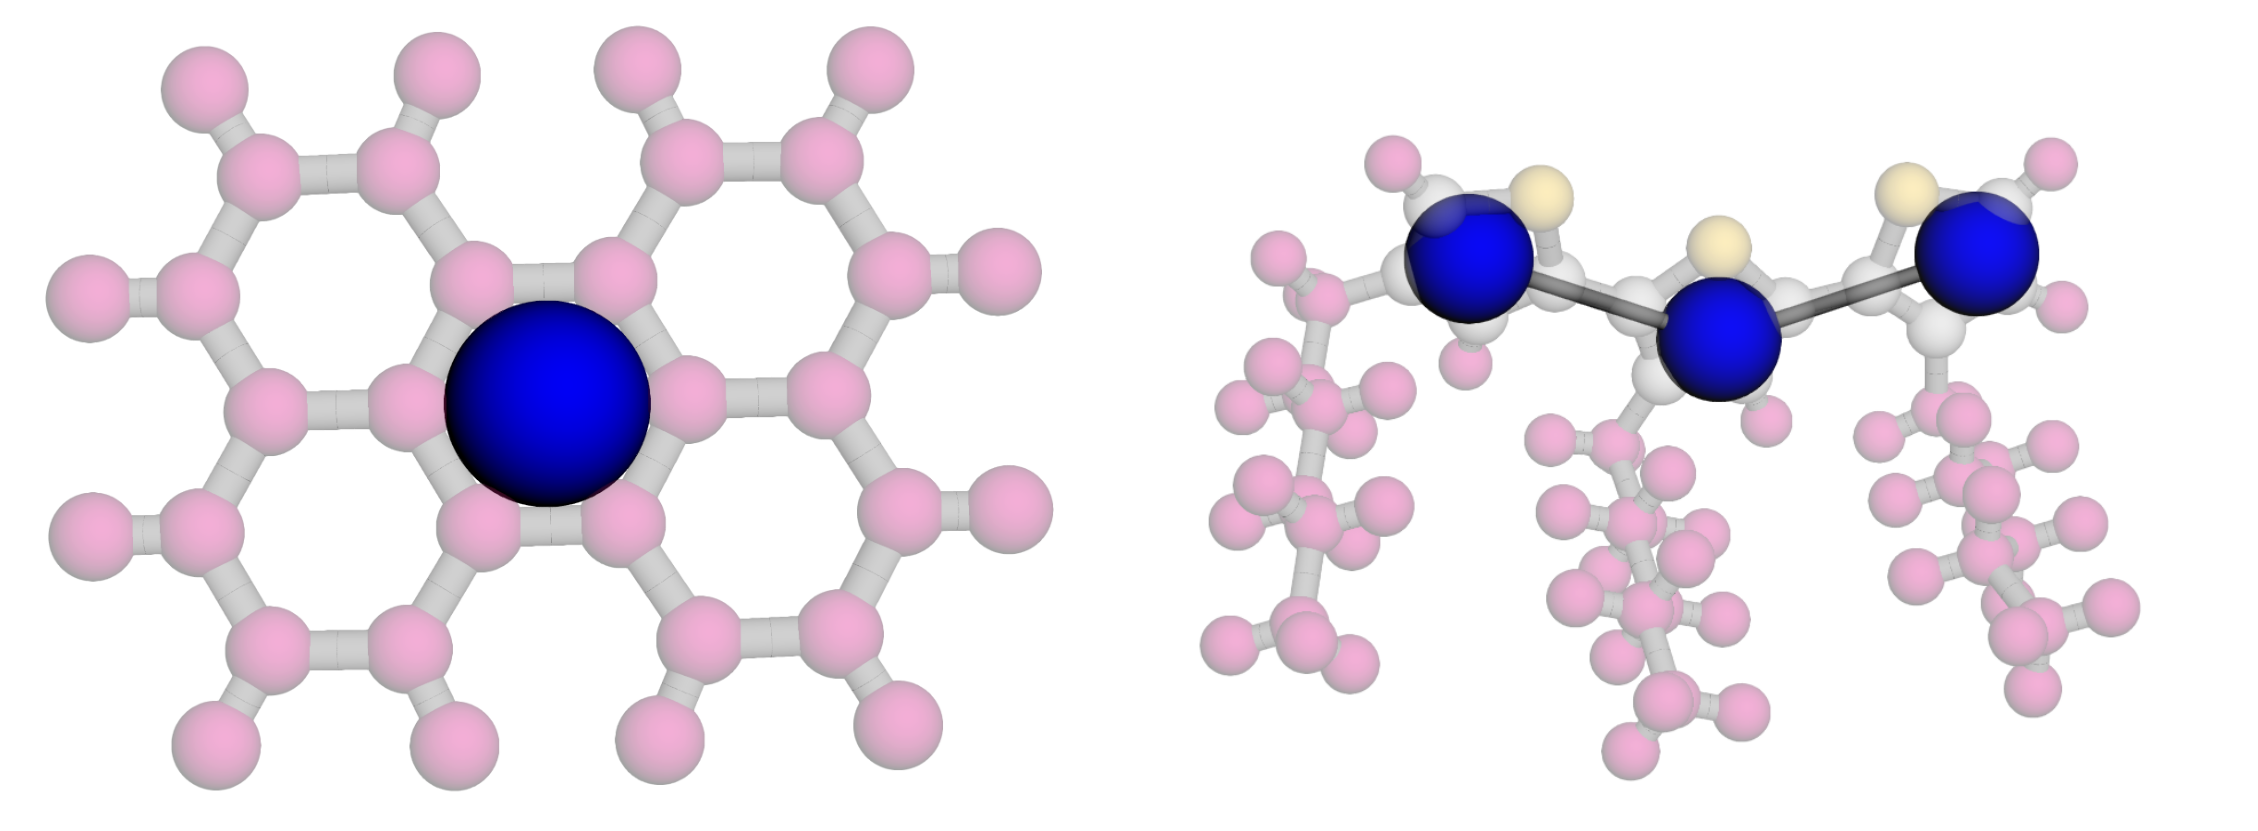
\includegraphics[width=.6\linewidth]{src/figures/FF_figs/per_p3ht_CG.png}
    \caption{Blue spheres represent center-of-geometry positions used for RDFs and clustering criteria. Perylene (left), and P3HT (right).}
    \label{fig:p3ht_per_CG}
\end{figure}

To compare with prior work, we calculate an order parameter $\Psi$ as used by Miller et al.~ \cite{miller_optimization_2018}that measures the fraction of perylene molecules--or monomers for P3HT--belonging to clusters of at least size 6.
Two perylene molecules--or two thiophene rings for P3HT--are considered clustered if their centers are within 6\AA~and the best-fit planes through each moiety are within 10 degrees of being parallel.
The code for calculating RDFs, GIXS, $\Psi$ and phase diagrams is available at \url{github.com/madilynpaul/Espaloma-Validation}. 

\subsection{Integrating Espaloma parameterization into MoSDeF} 

Our simulation workflows are built around MosDeF tools\cite{cummings_opensource_2021}, in particular \texttt{mBuild} \cite{Klein_mbuild} whose \texttt{mbuild Compound} objects are incompatible with the \texttt{openMM Molecule} objects expected by \esp.
To incorporate \esp~into MoSDef workflows we develop a helper function termed ``\texttt{BondWalker}'' that can convert \texttt{mbuild Compounds} into \texttt{openMM Molecules} (\autoref{esp_diagram}).
This workflow fits into the overall MD workflow (Section 4.2, \autoref{MD-Diagram}) within Step 4. 
\begin{figure}
    \centering
    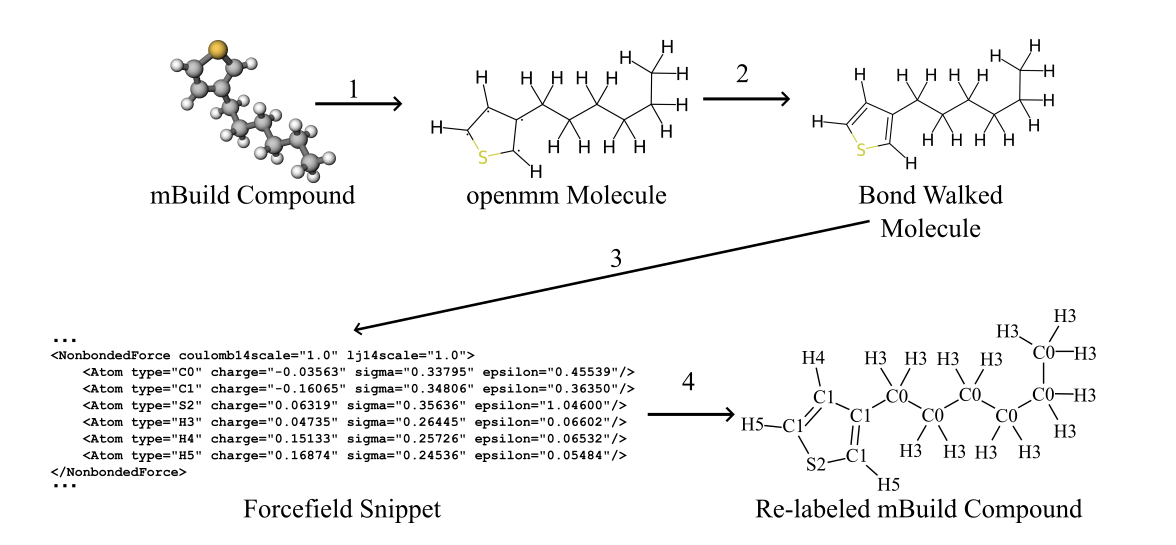
\includegraphics[width=1\linewidth]{src/figures/FF_figs/esp_fig.png}
    \caption{Overall \esp-\texttt{MosDeF} workflow. (1) \texttt{mBuild} compounds are used to create the topology of an \texttt{openMM} molecule, (2) \texttt{BondWalker} uses octet rules to determine double bonds in the \texttt{openMM} molecule. (3) \esp~generates forcefield parameters for the \texttt{openMM} molecule. (4) The \espff~forcefield is used to re-type the \texttt{mBuild} compound for use in \texttt{HOOMD-Blue} simulations.}
    \label{esp_diagram}
\end{figure}
The general procedure is: \textbf{(1)} Create an \texttt{openMM Molecule} topology from connectivity information of the \texttt{mBuild Compound} to be parameterized. 
\textbf{(2)} Rebuild the missing double and triple bonds in the \texttt{openMM Molecule} using the \texttt{BondWalker} function (See \autoref{bond_walk}). 
\textbf{(3)} Pass the \texttt{``BondWalked''} molecule to \esp for forcefield parameterization, writing these parameters to a forcefield \texttt{xml} file.
\textbf{(4)} Use the atom labels given by \esp to rename the atoms in our \texttt{mBuild Compound}. 
This last step ensures that the correct parameters will be applied to the corresponding atoms. 
A full tutorial of \esp~forcefield and typed \texttt{mBuild Compound} generation can be found at \url{github.com/madilynpaul/Espaloma-Validation}. 
%\begin{figure}[ht]
\begin{figure}
    \centering
    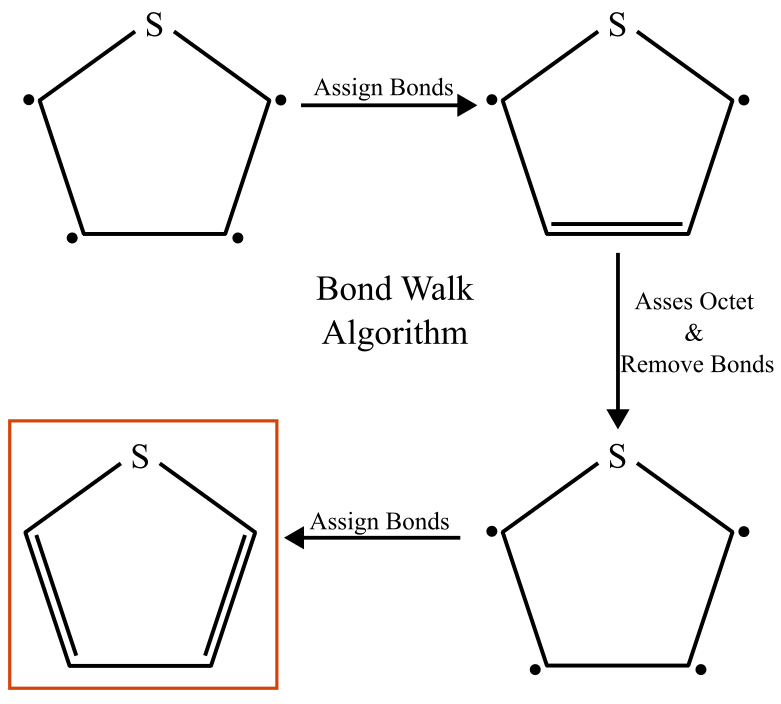
\includegraphics[width=0.5\linewidth]{src/figures/FF_figs/bondwalk_algorithm.png}
    \caption{Double- and triple-bond information that is missing from \texttt{mBuild} compounds is retrieved via \texttt{BondWalker} by iteratively checking whether the octet rules can be satisfied for all atoms after incrementing the bond character adjacent to atoms with unsatisfied octets.
}
    \label{bond_walk}
\end{figure}

%%%%%%%%%%%%%%%%%%%%%%%%%%%%%%%%%%%%%%%%%%%%%%%%%%%%%%

\section{Results and Discussion}
Here we report on the differences between the \espff~, \texttt{GAFF}, and \oplsff~parameters followed by a comparison between \espff~generated morphologies and \oplsff~morphologies generated in prior work.

\subsection{Espaloma vs OPLS-UA and GAFF}
The nonbonded pair interaction for perylene and P3HT are presented in \autoref{sigma_epsilon_comparison_table}, where they are compared against \oplsff~and \texttt{GAFF} parameters. 
\begin{table}[h!]
    \centering
    \caption{Lennard-Jones diameters $\sigma$ and well-depths $\epsilon$ generated by \texttt{espaloma} in the present work, and \texttt{OPLS-UA} and \texttt{GAFF}.}
    \begin{tabular}{c c c c|c c c} 
    & \multicolumn{3}{c}{$\sigma$ (\AA)} &  \multicolumn{3}{c}{$\epsilon$ (kJ/mol)}  \\
    \hline
        &  C1      &   C0      &   S &   C1      &   C0      &   S   \\
    \hline
    \texttt{Espaloma}    &   3.481   &   3.380   &   3.564  & 0.3635  & 0.4554  & 1.046   \\
    \texttt{OPLS-UA}     &   3.436   &   3.905   &   3.436  & 0.4602  & 0.7113  &  1.339   \\
    \texttt{GAFF}        &   3.3997  &   3.3997  &   3.564  & 0.3598  & 0.4577  &    1.046   \\
    \end{tabular}
    \label{sigma_epsilon_comparison_table}
\end{table}
We first consider the LJ $\sigma$ values, and note that \oplsff~is somewhat of an outlier, with much larger C0 diameters, while \espff~and \texttt{GAFF} are similar to each other. 
The \espff~C1's are slightly larger than both \oplsff~and \texttt{GAFF}, while the \espff~C0's are slightly smaller than \texttt{GAFF}.
\texttt{GAFF} and \espff~agree on the diameter of S atoms in P3HT.
We next consider the $\epsilon$ values and note that \espff~is very similar to \texttt{GAFF} once again, with \oplsff~as the outlier.

Normalizing the $\epsilon_{C1}$ and $\epsilon_{C0}$ values by $\epsilon_{S}$ provides a clearer picture of the range of attractions in each model than simple comparison the absolute values of each $\epsilon$.
For \espff, $\epsilon_{C1}/\epsilon_{S}=0.3475$, is nearly identical to that of \oplsff: $\epsilon_{C1}/\epsilon_{S}=0.3437$.
For C0, \espff~$\epsilon_{C0}/\epsilon_{S}=0.4353$, is about 20\% weaker than that of \oplsff: $\epsilon_{C0}/\epsilon_{S}=0.5312$.
To briefly summarize, the C1 parameterizations are close-but-not identical between \espff~and \oplsff, so we expect perylene simulations to be similar between the two models.
However, because the $\epsilon_{C1}/\epsilon_{S}$ and $\epsilon_{C0}/\epsilon_{S}$ ratios and C0 $\sigma$ values vary significantly between \espff~and \oplsff, it is unclear whether P3HT morphologies and phase behavior with \espff~will match those generated previously with \oplsff.

We perform MD simulations of each molecule to compare morphologies generated with the present \espff~parameterization against those previously generated with \oplsff.
A summary of simulation state points and units for each molecule is provided in \autoref{sim_parameters}. 
These statepoints are chosen to replicate structures sampled in prior work from Miller et al.\cite{miller_optimization_2018}.
Each temperature range encompasses the solid-liquid transition temperatures of approximately 500 K and 550 K for P3HT and perylene, respectively. 
The density ranges are chosen with respect to previous MD studies as well as experimental thin-film studies for P3HT\cite{newbloom2012structure}. 
We expect to observe various phases (ordered, liquid, vapor, disordered) over this range of statepoints.

\begin{table}
  \centering
    \caption{A list of statepoints used in the P3HT and perylene simulations, as well as the base units for each simulation (\begin{math}\sigma , \epsilon , M\end{math}).}
  \begin{tabular}{c|c|c}
      & \textbf{P3HT} & \textbf{Perylene} \\
    \hline
    Temperature Range (K) & [60.4,304.4,427.7,608.9]& [49.8,248.8,497.7,746.5]\\
    \hline
    Density Range (g/cm$^3$) & [0.25,0.5,1.0] & [0.5,1.0,1.5]\\
    \hline
    N & 100 & 250 \\
    \hline
    dt & 0.0003 & 0.0001 \\
    \hline
    M (amu) & 32.06 & 12.011 \\
    \hline
    \(\sigma\) (\AA)& 3.56 & 3.40 \\
    \hline
    \(\epsilon\) (kJ/mol)& 1.046 & 0.360\\
    \hline
    N\textsubscript{monomers}& 15 & 1 \\
  \end{tabular}
  \label{sim_parameters}
\end{table}

\subsection{Perylene} %Polish.
The ordering ($\Psi$) of perylene modeled with \espff~ as a function of temperature and density is summarized in \autoref{per_phase_diagram}.
Consistent with Ref.~\citep{miller_optimization_2018}, the most ordered structure (T = 250 K, $\rho$ = 0.5 g/cm$^3$) exhibits significant $\pi$-stacking, which is visible in \autoref{Per_snapshot}. 
At lower temperatures, we observe a transition from highly ordered to less ordered as the density increases, also in agreement with prior work.
This is due to the steric hindrance of having a high number of molecules in a restricted volume is observed in prior work.
\begin{figure}[ht]
    \centering
    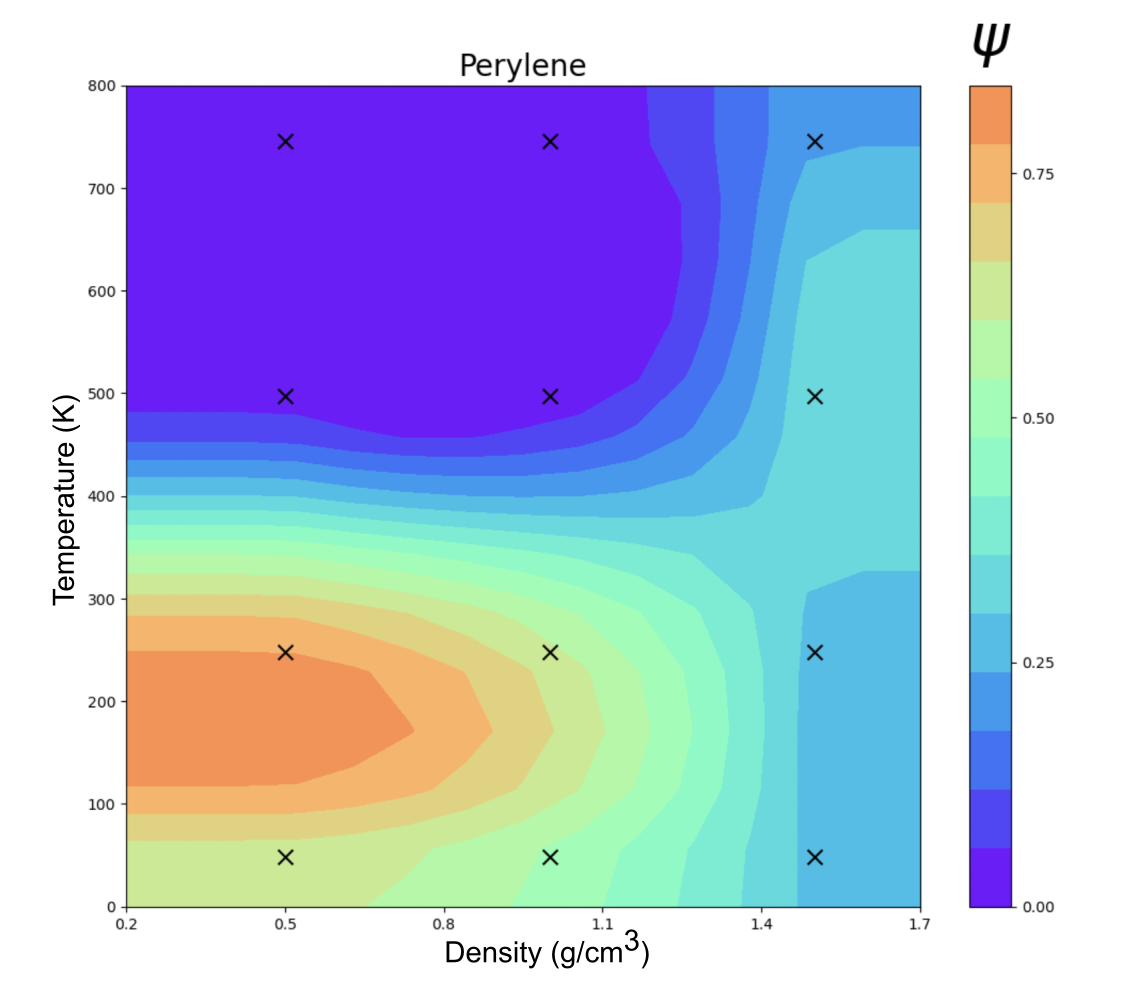
\includegraphics[width=0.6\textwidth]{src/figures/FF_figs/perPD.png} % 
    \caption{Temperature vs density clustering order parameter ($\Psi$) phase diagram of perylene at 12 statepoints.}
    \label{per_phase_diagram}
\end{figure}
\begin{figure}[h!]
    \centering
    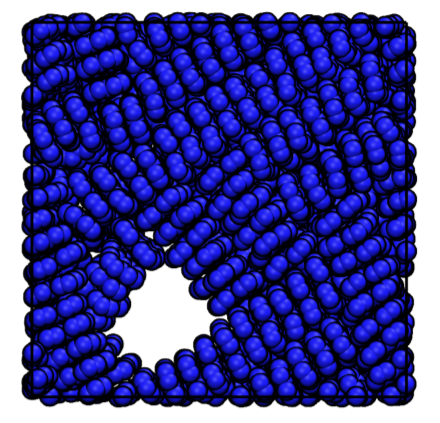
\includegraphics[width=0.35\linewidth]{src/figures/FF_figs/per_snapshot.png}
    \caption{Snapshot of perylene taken from the most ordered morphology at a density of 0.5 g/cm$^3$ and temperature of 248.8 K.}
    \label{Per_snapshot}
\end{figure}
However, the order-disorder transition temperature observed here around 470 K is roughly 0.79 that of the 600 K in Ref.~\citep{miller_enhanced_2017} and Botoshansky et al\cite{botoshansky2003towards}.
This is explained by the difference in base unit between \esp~and \texttt{OPLS-UA} perylene forcefields: Both models have only C1 atomtypes but $\epsilon_{OPLS-UA}=0.4602$ kJ/mol and $\epsilon_{ESP-UA}=0.3635$ kJ/mol. 
The ratio between these two energy units $\frac{\epsilon_{ESP-UA}}{\epsilon_{OPLS-UA}}=0.79$ matches the transition temperature discrepancy.
That is, in dimensionless units, there is no significant difference in the temperature-density phase diagrams between the two forcefields.
Given that the energy unit of \oplsff~gives an order-disorder transition temperature in agreement with experiments, this suggests that the absolute \espff~energy units may benefit from empirical rescaling.

A comparison to the RDFs reported in Miller, et al.~at density of 1.7 g/cm$^3$ and the present work shows good agreement in short-range ordering as a function of temperature.
 First peak locations for the ordered systems in the \espff~and \oplsff~RDF's align at 3.8 \AA. 
 First peak locations in the disordered systems produced by \espff~and \oplsff~both appear at approximately 4 \AA. 
 Differences in peak intensity can be explained by the difference in density between the two systems. 
 As expected, the RDFs calculated  at higher temperatures show less intense peaks. 
 We observe high ordering at 50 K and 249 K, in correspondence to the RDF reported by Miller, et al.~
 We observe consistent RDF peak locations between the \espff~simulation results at temperature of 498 K and the \oplsff~simulation results reported in the droplet phase by Miller, et al.~ 
\begin{figure}[h!]
    \centering
    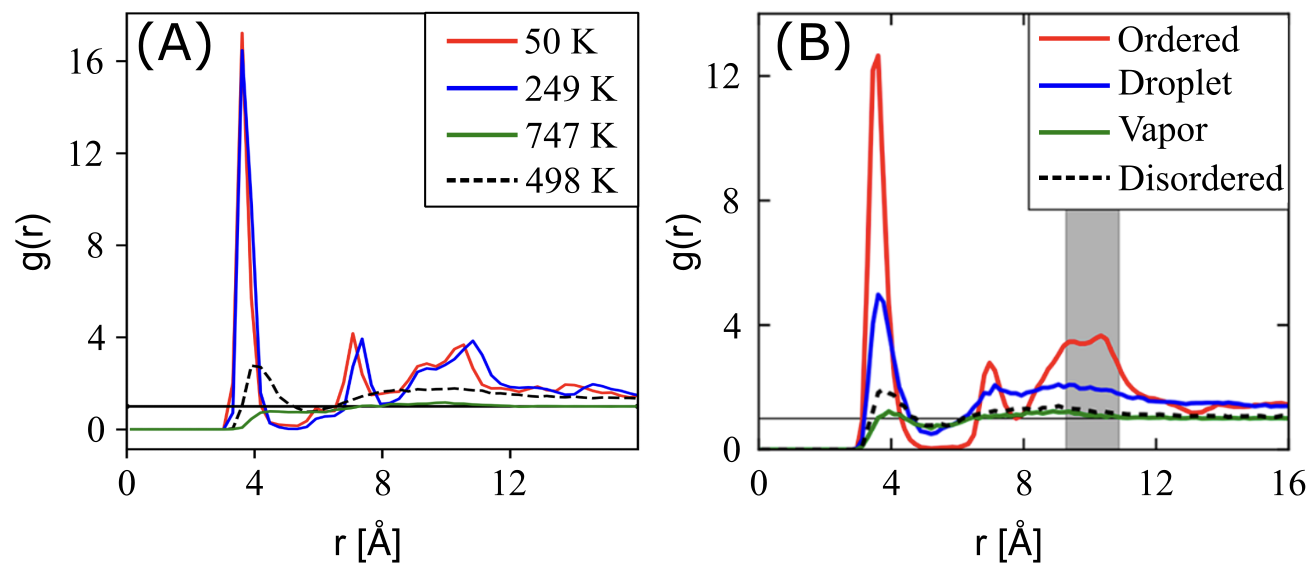
\includegraphics[width=.75\textwidth]{src/figures/FF_figs/per_rdf.png}
    \caption{(A) Radial distribution function (RDF) of Perylene at various temperatures at a density of 0.5g/cm$^3$ generated from an \espff~predicted morphology. (B) RDF of perylene in various phases generated from an \oplsff~predicted morphology. \oplsff~RDF published by Miller, et al.~at Ref \citep{miller_enhanced_2017}.}
    \label{per_rdf}
\end{figure}

Long-range order is measured via simulated GIXS at temperature of 250 K and density of 0.5 g/cm$^3$. 
Bragg reflections are observed along both the x and y axes, indicating significant long-range order and close packed columns, which are observed in \autoref{Per_snapshot}. 
One major difference between the \espff~generated GIXS pattern here and the \oplsff~pattern in prior work is the $q_y$ location of the 001 reflection: From \oplsff~the 001 reflection occurs around $0.8 A^{-1}$, while with \espff~here $q_y=1.9 A^{-1}$ in better agreement with Ishii and Miyasaka\citep{Ishii}.
\begin{figure}[h!]
    \centering
    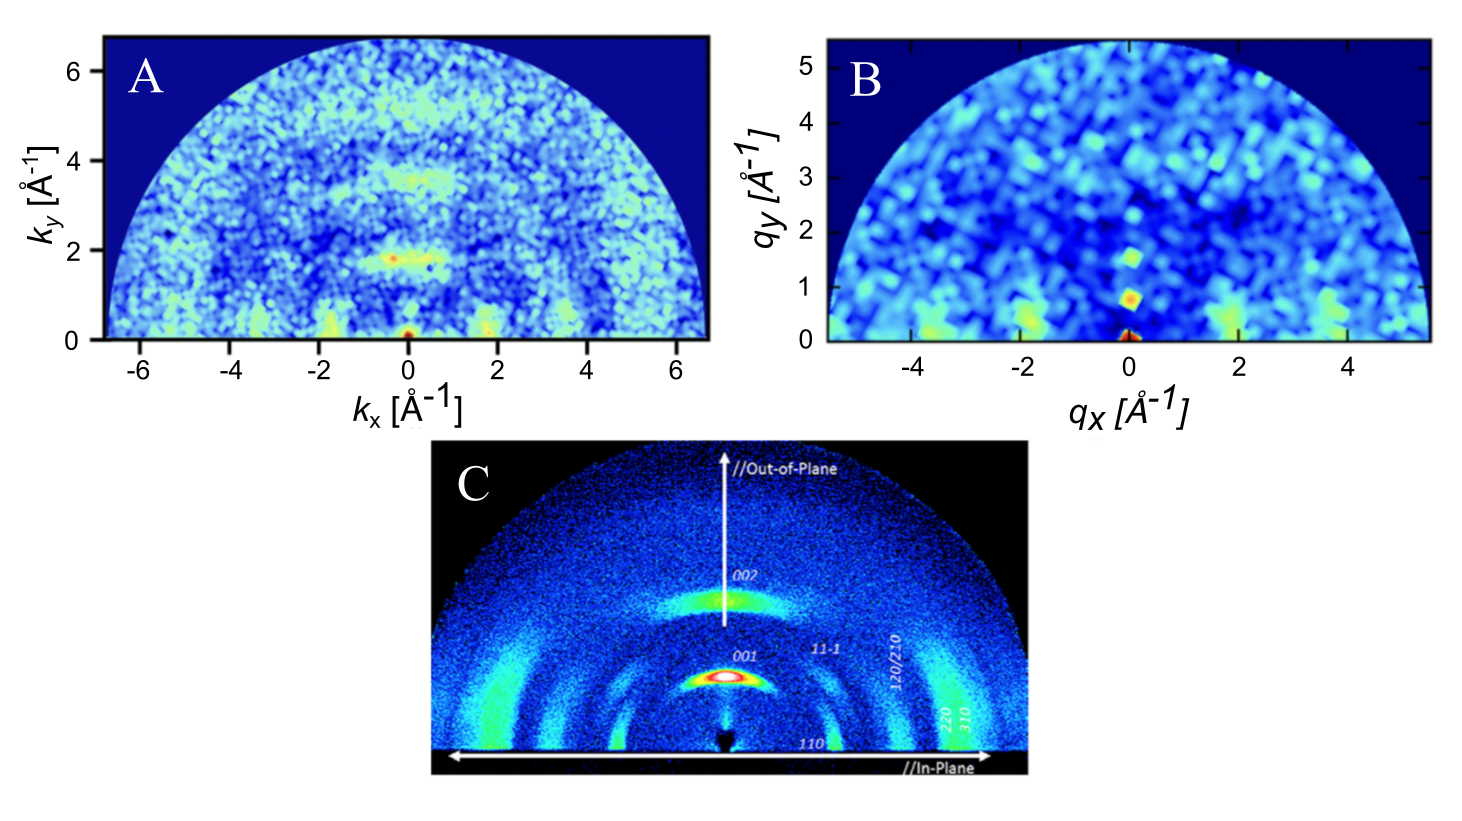
\includegraphics[width=1\textwidth]{src/figures/FF_figs/per_gixs.png} 
    \caption{(A) Grazing incident x-ray scattering pattern of Perylene generated from an \espff~morphology. (B) GIXS pattern of Perylene generated from an \oplsff~morphology. \oplsff~GIXS pattern published by Miller, et. al. at Ref \citep{miller_enhanced_2017}. (C) Experimental XRD pattern for $\beta$-perylene, reproduced with permission from Ishii, et al.~ at Ref \citep{ishii_fully_2014}. Copyright 2014 AIP Publishing LLC.}
    \label{Per_GIXS}
\end{figure}
To briefly summarize, modeling perylene with \espff~parameterization results in phase behavior and short-range ordering in agreement with prior \oplsff~work, however long-range ordering as measured by GIXS matches experiments better, while the base energy unit of \oplsff~gives better temperature correspondence.

%%%%%%%%%%%%%%%%
\subsection{Poly-3-Hexylthiophene (P3HT)}
\begin{figure}[h!]
    \centering
    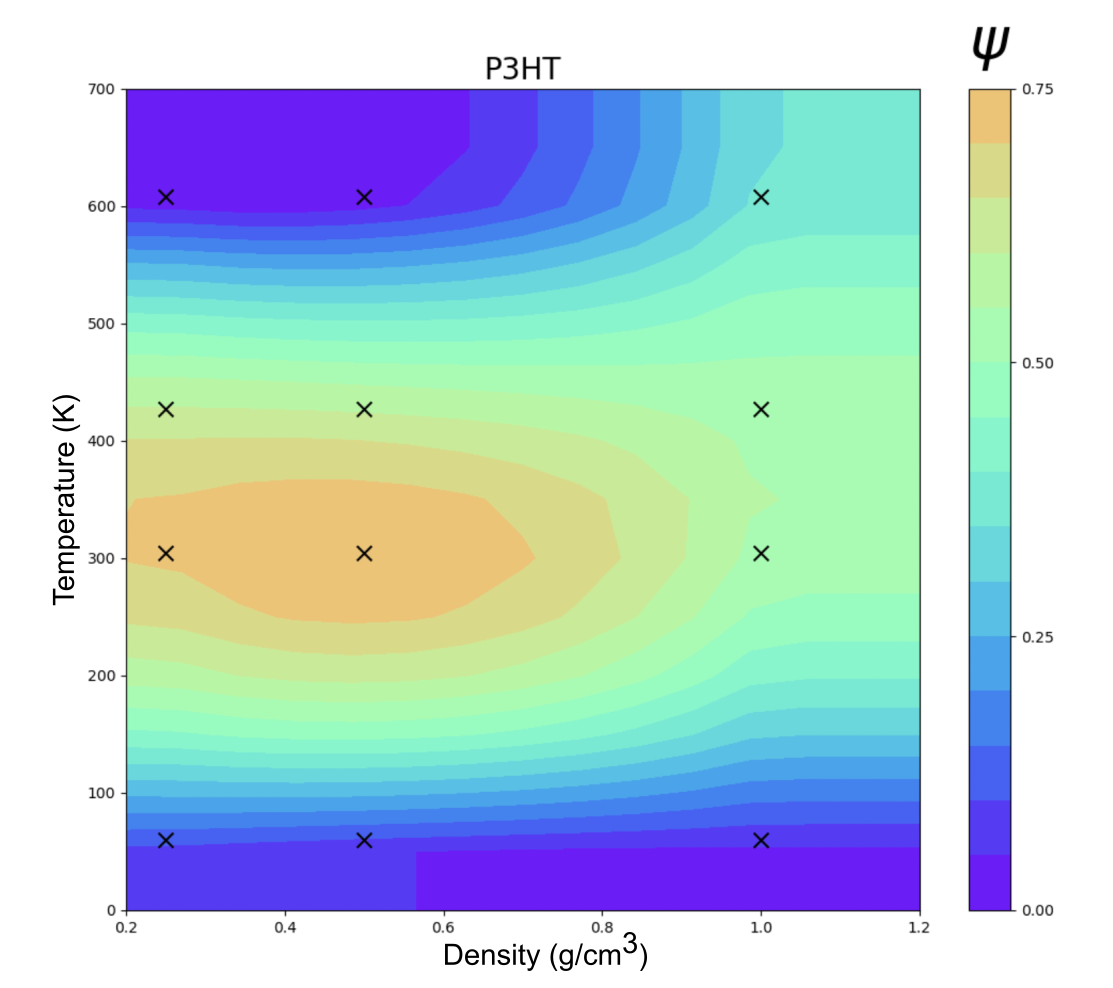
\includegraphics[width=0.6\textwidth]{src/figures/FF_figs/p3htPD.png} % Replace 'example-image' with your image file name and path
    \caption{Temperature vs density clustering order parameter ($\Psi$) phase diagram of P3HT at 12 statepoints.}
    \label{p3ht_phase_diagram}
\end{figure}
\autoref{p3ht_phase_diagram} shows the clustering order parameter ($\Psi$) phase diagram of P3HT as a function of temperature and density. 
 As observed with perylene, the transition temperatures are too low relative to experiments, and this is again explained by the differences in $\epsilon$ units between \espff~and \oplsff.
 \espff~gives an $\epsilon$ of 0.4554 kJ/mol for the aliphatic side chain carbons of P3HT, while \oplsff~uses an $\epsilon$ of 0.7113 kJ/mol. 
 This creates more ordered side chains in the \oplsff~simulations in comparison to the \espff~simulations. 
 This observation is supported by the work in Reference \citep{marsh_controlling_2014}, stating that lower the $\epsilon$ values for side chains of P3HT monomers results in lamellar structures at lower temperatures than if the $\epsilon$ was higher \citep{marsh_controlling_2014}. 
\begin{figure}[h!]
    \centering
    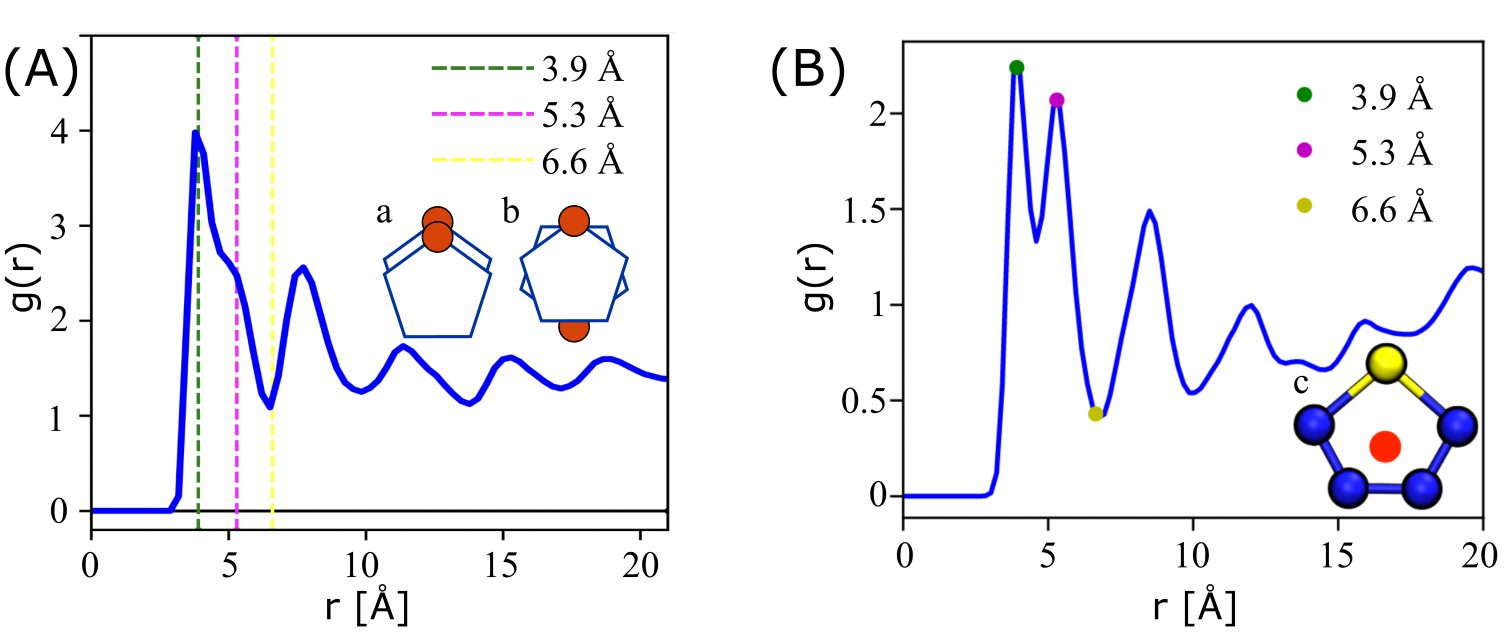
\includegraphics[width=.75\textwidth]{src/figures/FF_figs/p3ht_rdf.png}
    \caption{(A) Radial distribution function (RDF) of P3HT at a temperature of 304 K and a density of 0.5g/cm$^3$ generated from an \espff~predicted morphology. 
 (B) RDF of P3HT generated from an \oplsff~predicted morphology. 
 \oplsff~RDF published by Miller, et al.~in Ref \citep{miller_optimization_2018}.}
    \label{P3HT RDF}
\end{figure}
\autoref{P3HT RDF} shows the radial distribution function of \espff~P3HT (left) and \oplsff~P3HT (right). 
 The \espff~RDF is generated at a temperature of 304 K and a density of 0.5g/cm$^3$. 
 Three vertical dashed lines in the \espff~RDF correspond to the local maxima and minima highlighted in the \oplsff~RDF. 
 The first peak in each corresponds to the aligned $\pi$-stacking of the thiophene rings, shown in \autoref{P3HT RDF}a. 
 The second peak aligns with the anti-aligned $\pi$-stacking of the thiophene rings, shown in \autoref{P3HT RDF}b. 
 The \oplsff~RDF is calculated using the geometric center of thiophene ring, shown in \autoref{P3HT RDF}c. 
 The \espff~RDF is calculated using only the S-S interactions, excluding those in the same chain. 
 The sulfurs were chosen for the \espff~RDF because they are central to the ring, hold the most mass and have the largest radius. 
\begin{figure}[h!]
    \centering
    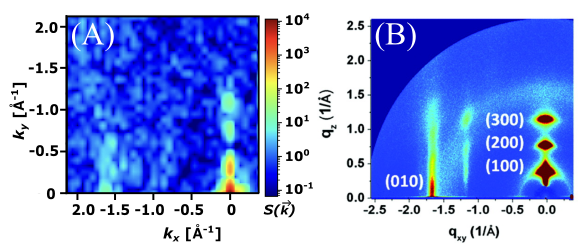
\includegraphics[width=.8\textwidth]{src/figures/FF_figs/p3htGIXS&exp.png}
    \caption{(A) Grazing Incident X-ray Scattering Pattern of P3HT at 0.5 g/$cm^3$ and 304 K generated using \espff. (B) Corresponding experimental scattering pattern of P3HT. Reprinted (adapted) with permission from Ko, et al.~in Ref \citep{p3ht_experimental}. Copyright 2012 American Chemical Society.}
    \label{p3ht_GIXS}
\end{figure}
\par The GIXS scattering pattern of the most ordered structure (0.5 g/cm$^3$, 304 K) displays significant correlation to the experimental scattering pattern of P3HT (\autoref{p3ht_GIXS}). 
 Peaks are observed at approximately 1.65 \AA \textsuperscript{-1} corresponding to the (010) plane, as well as peaks along the (100) plane spaced approximately 0.3 \AA \textsuperscript{-1} apart. 
 This correlation between experiment and simulation confirms that the \espff~is able to responsibly parameterize and represent the P3HT polymer in simulations. 
 The lamellar structure represented by the scattering pattern in \autoref{p3ht_GIXS} is shown in \autoref{p3ht_lamellar}. 
\begin{figure}[hbt!]
    \centering
    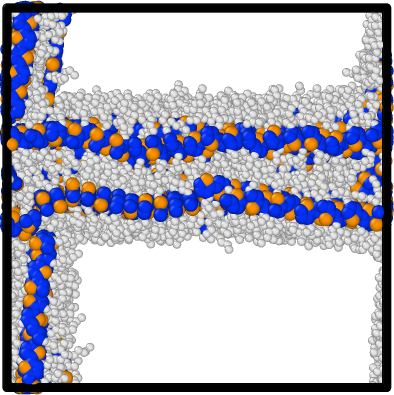
\includegraphics[width=0.5\textwidth]{src/figures/FF_figs/p3ht_0.5den_2.42kT.png}
    \caption{Snapshot of P3HT's most ordered morphology at a density of 0.5 g/cm$^3$ and temperature of 304 K.}
    \label{p3ht_lamellar}
\end{figure}


%%%%%%%%%%%%%%%%%%%%%%%%%%%%%%%%%%%%%%%%%%%%%%%%%

\section{Conclusions}
We successfully incorporate \esp~forcefield generation into \texttt{MoSDeF} workflows for investigating organic molecule phase behavior via MD simulations. 
\esp~generates reasonable forcefield parameters for macromolecules with high aromaticity as well as for thiophene-based conjugated polymers as measured by GIXS, RDF, and phase behavior.
The GIXS scattering patterns for both perylene and P3HT showed long range order that was consistent with published experimental work, and in the case of perylene has better agreement than \oplsff in matching the length scale of the 100 reflection. 
One caveat is that the absolute energy units generated by \espff~may be too low for the molecules of interest.
Here we find that multiplying \espff~$\epsilon$ values by 1.26 to be in closer agreement with \oplsff~gives better agreement for P3HT and Perylene's experimental phase transitions between ordered and disordered phases.
Whether this rescaling rule is universal or is dependent upon the specific chemistries remains the subject of future work.
Nevertheless, the present observations inform confidence in using \esp~to quickly generate forcefields for molecules that are missing information in ``off-the-shelf'' forcefields like \oplsff~and \texttt{GAFF}, subject to the energy-rescaling caveat above.
We conclude that \esp~holds promise as a component in high-throughput screenings of organic molecules for phase behavior in systems from polymer thermoplastics to organic photovoltaics to macromolecular drug packing and more.
